
\item A long insulated copper wire is closely wound as a spiral of `N' turns. The spiral has inner radius `a' and outer radius `b'. The spiral lies in the X-Y plane and a steady current `I' flows through the wire. The Z-component of the magnetic field at the center of the spiral is
    \begin{center}
        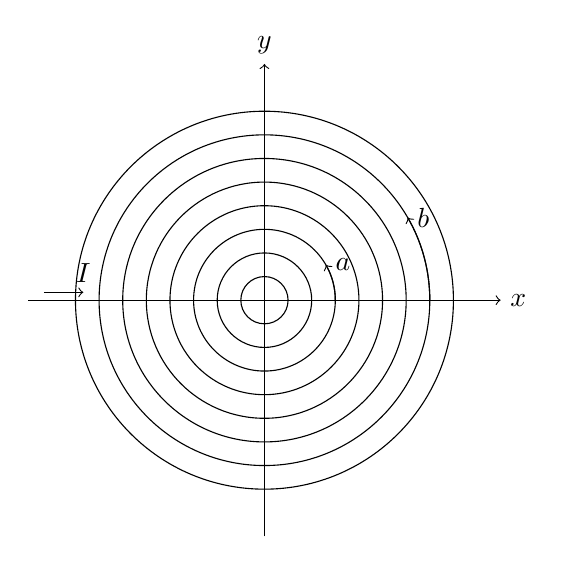
\begin{tikzpicture}
        % Draw the x and y axes
        \draw[->] (-3,0) -- (3,0) node[right] {$x$};
        \draw[->] (0,-3) -- (0,3) node[above] {$y$};

        \foreach \r in {0.3,0.6,...,2.7} {
            \draw (\r,0) arc (0:360:\r);
        }

        % Labels for inner and outer radius
        \draw[->] (0.9,0) arc (0:30:0.9) node[right] {$a$};
        \draw[->] (2.1,0) arc (0:30:2.1) node[right] {$b$};

        % Indicate the current direction
        \draw[->] (-2.8,0.1) -- (-2.3,0.1) node[above] {$I$};

        \end{tikzpicture}
    \end{center}
    \begin{tasks}(2)
        \task $\frac{\mu_0 N I}{2(b-a)} \ln\left(\frac{b}{a}\right)$
        \task $\frac{\mu_0 N I}{2(b-a)} \left[\ln\left(\frac{b+a}{b-a}\right)\right]$
        \task $\frac{\mu_0 N I}{2b} \ln\left(\frac{b}{a}\right)$
        \task $\frac{\mu_0 N I}{2b} \ln\left(\frac{b+a}{b-a}\right)$
    \end{tasks}
